% This is a copy version from https://github.com/thanhhungqb/thesis-template
% Please do not modified this project, when you want to start writing, make a clone of it for your own (Please read README.md)

\documentclass[12pt,a4paper,oneside]{book} % twoside for draf

%\usepackage{babel}
\usepackage[utf8]{vietnam}
\usepackage{times}
\usepackage{graphicx}

\usepackage{mathptmx}	% same Time New Roma
%\renewcommand{\rmdefault}{phv} % Arial
%\renewcommand{\sfdefault}{phv} % Arial

\usepackage{fancyhdr}
\usepackage{algorithm2e}
\usepackage{commath}
\usepackage{bkthesis}
\usepackage{amsmath}
\usepackage{amsfonts}
\usepackage{amssymb}
\usepackage{url}

\crname{LUẬN VĂN TỐT NGHIỆP ĐẠI HỌC}
\cstuname{SVTH: Đào Huỳnh Trung }
\ctname{\fontsize{18}{18}\selectfont SỬ DỤNG ĐIỆN TIM TRONG XÁC ĐỊNH BẤT THƯỜNG Ở NGƯỜI SỬ DỤNG HỌC MÁY}

\csCouncil{}
\csSupervise{TS. Nguyễn Đức Dũng\\
            TS. Huỳnh Tường Nguyên
}
% \csReviewer{TS. Nguyễn Đức Dũng}
\cttime{01/04/2019}

\thesislayout

\begin{document}
%-	Bìa cứng - màu xanh dương, chữ mạ vàng (xem mẫu đính kèm)
%-	Trang tên (tờ lót): chất liệu giấy, nội dung giống như bìa LV
%-	Ở gáy LV: in nhan đề LV (có thể in tóm tắt nếu nhan đề quá dài), size 15 – 17
%-	Phiếu Nhiệm vụ LV, chấm điểm Hướng dẫn & Phản biện (đã ký): nhận từ GVHD & GVPB sau khi bảo vệ (theo lịch hẹn).
%-	Lời cam đoan
%-	Lời cảm ơn/ Lời ngỏ
%-	Tóm tắt LV
%-	Mục lục
%-	Danh mục, bảng biểu, hình ảnh, ... (nếu có)
%-	Nội dung LV
%-	Danh mục TL tham khảo
%-	Phụ lục (nếu có)

\coverpage

\frontmatter

% add content here
%-	Lời cam đoan
% \begin{declaration}
%  	Tôi xin cam đoan...
%  \end{declaration}

%-	Lời cảm ơn/ Lời ngỏ
% \begin{acknowledgments}
% 	Tôi xin chân thành cảm ơn ...
% \end{acknowledgments}

%-	Tóm tắt LV
% \begin{abstract}
% 	Tóm tắt luận văn ...
% \end{abstract}	
	
\tableofcontents
%\listofsymbols
% \listoftables
% \listoffigures
%\listofalgorithms


\mainmatter

\fancyhead{}  % Clears all page headers and footers
%\rhead{\thepage}  % Sets the right side header to show the page number
%\lhead{}  % Clears the left side page header
%\fancyfoot[positions]{footer}
\renewcommand{\footrulewidth}{0.4pt}

\pagestyle{fancy}  % Finally, use the "fancy" page style to implement the FancyHdr headers

\chapter{Giới thiệu}
\newpage

\section{Đặt vấn đề}
Theo ước tính của Tổ chức Y tế thế giới, hàng năm trên thế giới có khoảng 17,5 triệu người tử vong do các bệnh liên quan đến tim mạch và số bệnh nhân tim mạch tích lũy ngày một nhiều. Theo dự báo của Hội Tim mạch Việt Nam, khoảng 20\% dân số nước ta mắc bệnh về tim mạch và tăng huyết áp. Tỷ lệ tăng huyết áp ở những người trẻ từ 25 tuổi đang gia tăng, chiếm 21,5\% tổng số ca mắc bệnh.Tuy nhiên, vẫn còn nhiều người thờ ơ, chủ quan và thiếu quan tâm đến sức khoẻ tim mạch của mình. Theo thống kê của Hội tim mạch Việt Nam, vào năm 1980, tỷ lệ mắc bệnh tim mạch ở tuổi 50 trở lên chỉ ở mức 11\%, thì đến năm 2009, tỷ lệ này lên đến 25\% và độ tuổi mắc từ 22 tuổi trở lên.\cite{baibao}\par

\section{Mục tiêu}
Vì thế việc phát hiện sớm những dấu hiệu bất thường của tim đóng vai trò rất quan trọng giúp giảm nguy cơ mắc các bệnh tim mạch. Trong đó một trong những phương pháp để phát hiện bệnh là đo điện tim. Những để đo điện tim thì một người phải vào các cơ sở y tế với các thiết bị chuyện dụng. Cách làm này tốn khá nhiều thời gian và tiền bạc. Trong khi đó nếu ta có thể thu thập tín hiệu điện tim từ các thiết bị IoT tiếp qua một hệ thống phân loại để phát hiện bất thường ở điện tim một cách nhanh chóng và tương đối chính xác sẽ góp phần giám thiểu nguy cơ mắc bệnh tim mạch. Mục tiêu của để tài là sử dụng một hệ thống phân loại sử dụng các kỹ thuật học sâu (Deep Learning) để phát hiện loại bất thường ở điện tim.


\chapter{Tổng quan về điện tâm đồ}
\thispagestyle{fancy}

\section{Những khái niêm cơ bản về điện tâm đồ}
\subsection{Định nghĩa}
Điện tâm đồ (ECG) là một đường cong ghi lại các biến thiên của các điện lực do tim phát ra trong khi hoạt động co bóp. Ngoài đo tốc độ và nhịp điệu của tim thì điện tâm đồ còn cung cấp thêm những bằng chứng gián tiếp về lưu lượng máu truyền đến tim. Một xung điện sẽ được tạo ra từ các tế bào trong buồng tim khi tim hoạt động và những tín hiệu khi những xung điện này theo một hệ thống dẫn truyền đi qua tim sẽ được điện tâm đồ ghi lại. Nhờ có điện tâm đồ mà các bác sĩ có thể phát hiện ra được những bệnh lý về tim như loạn nhịp tim, đau thắt ngực,…Thỉnh thoảng, việc tiến hành điện tâm đồ cũng được coi như một xét nghiệm thường quy tại các bệnh viện.
\begin{center}
    \begin{figure}[htp]
    \begin{center}
    %  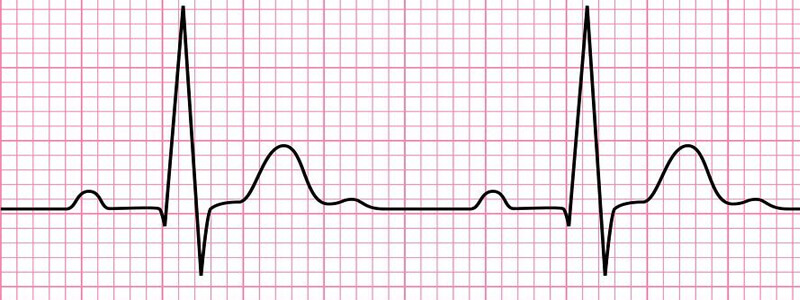
\includegraphics[scale=.]{image/week1/intro.jpg}
     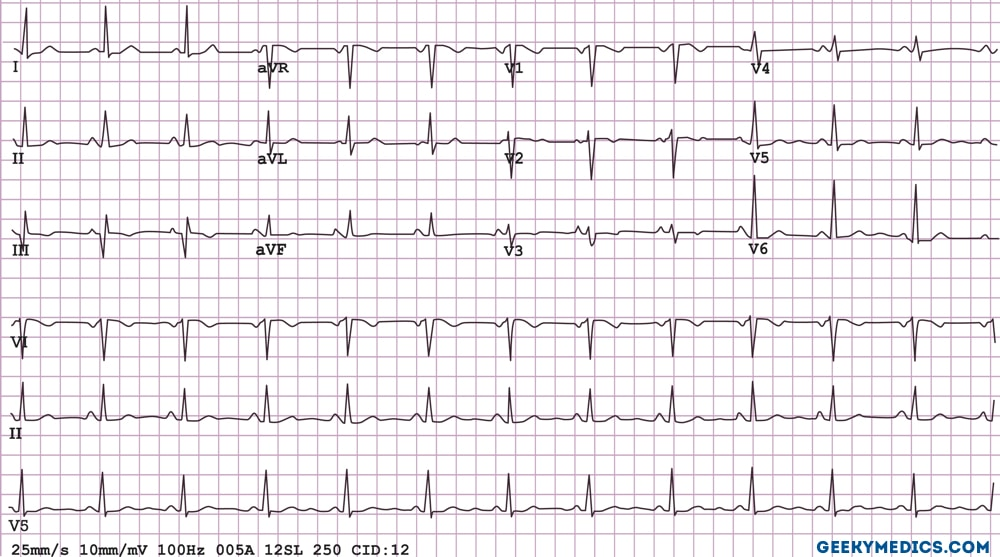
\includegraphics[scale=.35]{image/chapter1/Normal-ECG-SCALED-DOWN-WATERMARK.jpg}
    \end{center}
    \caption{Một đoạn điện tâm đồ }
    \end{figure}
\end{center}

\subsection{Lich sử hình thành điện tâm đồ}
\begin{itemize}
    \item 1887 - Augustus D. Waller (St Mary's Medical School, Luân Đôn) trình bày ECG đầu tiên trên người của Thomas Goswell, một người làm việc trong phòng thử nghiệm.
    \item 1893 - Willem Einthoven giới thiệu từ 'electrocardiogram' tại buổi họp của Hội Y Học Hà Lan (nhưng sau đó ông sửa lại rằng Waller là người đầu tiên dùng chữ này).
    \item 1895 - Einthoven cải tiến dụng cụ và công thức ghi điện, ghi được 5 thay đổi điện trong một nhịp tim, ông ghép chữ cho 5 thay đổi này (P, Q, R, S, T, U).
\end{itemize}

\subsection{Hoạt động điện của cơ tim và sự hình thành điện tâm đồ}
Do sự biến đổi hiệu thế giữa mặt trong và mặt ngoài màng tế bào cơ tim. Sự biến đổi hiệu thế này bắt nguồn từ sự di chuyển của các ion K + , Na + ,... từ ngoài vào trong tế bào và từ trong tế bào ra ngoài khi tế bào cơ tim hoạt động. Lúc này tính thẩm thấu của màng tế bào đối với các ion luôn luôn biến đổi. Do sự chênh lệch nồng độ hai bên màng tạo nên hiệu điện thế giữa hai bên màng (điện thế nghỉ).
\begin{center}
    \begin{figure}[htp]
    \begin{center}
     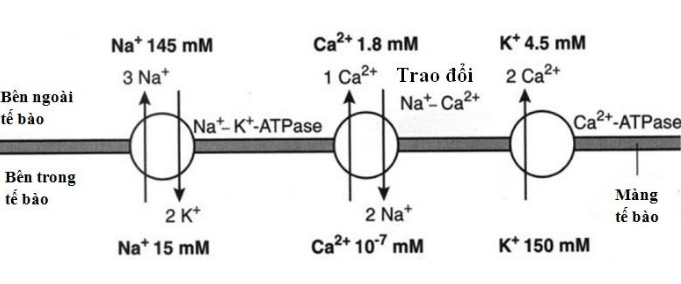
\includegraphics[scale=.4]{image/week1/h21.png}
    \end{center}
    \caption{Sự chênh lệch nồng độ của các ion Na, K, Ca trong cơ chế hình thành điện tâm đồ \cite{huongdanDTT}}
    \end{figure}
\end{center}\par
Tim người có 4 buồng để chứa và bơm máu. Hai phần nhỏ ở phía trên gọi là tâm nhĩ (vì trông giống lỗ tai). Hai phần dưới lớn hơn gọi là tâm thất. Máu theo tĩnh mạch từ cơ thể trở về tâm nhĩ phải, từ phổi trở về tâm nhĩ trái. Tâm nhĩ trái bóp bơm máu vào tâm thất trái, tâm nhĩ phải đưa máu vào tâm thất phải. Sau đó tâm thất phải bóp để bơm máu theo động mạch lên phổi và tâm thất trái bóp để bơm máu xuống cơ thể. Tim có khả năng hoạt động đều đặn và thứ tự như thế là nhờ một hệ thống các tế bào dẫn điện đặc biệt nằm trong cơ tim.\par
Trong tâm nhĩ bên phải có nút xoang nhĩ (sinoatrial node) gồm các tế bào có khả năng tự tạo xung điện (electric impulse). Xung điện này truyền ra các cơ chung quanh làm co bóp hai tâm nhĩ (tạo nên sóng P trên Điện Tâm đồ). Sau có dòng điện tiếp tục truyền theo 1 chuỗi tế bào đặc biệt tới nút nhĩ thất (atrioventricular node) nằm gần vách liên thất rồi theo chuỗi tế bào sợi Purkinje chạy dọc vách liên thất lan vào các cơ chung quanh (loạt sóng QRS) làm hai thất này co bóp. Sau đó xung điện giảm đi, tâm thất giãn ra (tạo nên sóng T).

\subsection{Các sóng cơ bản và sự hình thành phức bộ sóng}
Một chu kỳ tim biểu hiện trên điện tâm đồ là: sóng P, phức bộ QRS, sóng T, và sóng U (nếu có), hình dạng, thời gian kéo dài của sóng/phức bộ và cả thời gian giữa các thành phần với nhau đều có ý nghĩa đặc biệt quan trọng trong việc chẩn đoán.
\begin{center}
        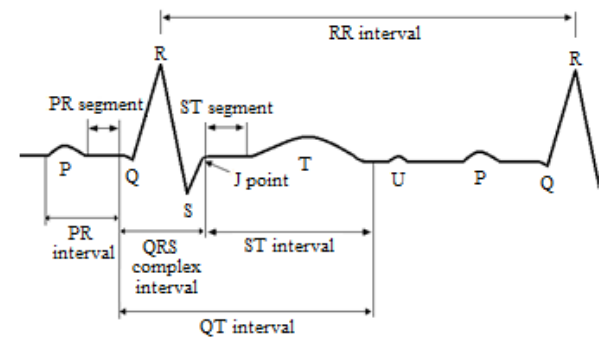
\includegraphics[scale=.4]{image/week1/h32.png}
        \begin{figure}[htp]
        \begin{center}
        \end{center}
        \caption{Tổng hợp những sóng cơ bản}
        \end{figure}
\end{center}

\subsubsection{Các sóng và phức bộ}
\textbf{Sóng P}\par
Sóng P hình thành do quá trình khử cực tâm nhĩ (cả nhĩ trái và nhĩ phải), bình thường biên độ của sóng P thường dưới 2mm (0.2mmV), và thời gian của sóng P là từ 0.08 đến 0.1 giây, việc tăng biên độ và kéo dài thời gian của sóng gợi ý đến một tình trạng tâm nhĩ lớn (tăng biên độ gợi ý lớn nhĩ phải. thời gian khử cực kéo dài gợi ý đến lớn nhĩ trái).\par
\textbf{Phức bộ QRS}\par
Phức bộ QRS thể hiện quá trình khử cực của tâm thất, tùy vào chiều khử cực và vị trí đặt điện cực mà trên giấy ghi sẽ cho thấy các phức bộ khác nhau, ưu thế sóng R hay S, bình thường QRS kéo dài từ 0.06 đến 0.1 giây.
\begin{itemize}
    \item Sóng Q là sóng âm đầu tiên của phức bộ QRS, sóng Q trên bệnh nhân bình thường thường nhỏ và ngắn (hình thành do quá trình khử cực vách liên thất), một sóng Q sâu (biên độ âm lớn) và kéo dài cho thấy một tình trạng hoại tử cơ tim (Trong nhồi máu cơ tim cũ hay nhồi máu cơ tim không có ST chênh lệch).
    \item Sóng R là sóng dương đầu tiên của phức bộ, và sóng âm sau nó là S, đây là hai sóng hình thành do khử cực thất, về bản chất là giống nhau, nếu điện cực đặt ở vị trị chiều khử cực hướng đến thì sóng R sẽ ưu thế, như trong chuyển đạo DII, V5, V6. Sóng R sẽ ưu thế hơn nếu chiều khử cực đi xa vị trí đặt điện cực như V1, V2.
\end{itemize}
\par
\textbf{Sóng T}\par
Là sóng theo sau phức bộ QRS, thể hiện quá trình tái cực muộn của 2 tâm thất, sóng T có giá trị rất lớn trong việc nhận định một tình trạng cơ tim thiếu máu.\par
\textbf{Sóng U}\par
Nguồn gốc sóng U vẫn chưa điện xác định rõ ràng, các giả thuyết đặt ra là:
\begin{itemize}
    \item Tái cực chậm sợi Purkinje.
    \item Tái cực kéo dài giữa cơ tim tế bào M (mid-myocardial cell).
    \item Sau kết quả điện thế của trương lực cơ trong các thành tâm thất.
\end{itemize}
Bình thường không thấy sóng U trên điện tâm đồ, nếu có thì là sóng nhỏ sau sóng T, sóng U đảo ngược hay nhô cao nhọn gặp trong rất nhiều loại bệnh lý tim (bệnh mạch vành, tăng huyết áp, bệnh van tim, tim bẩm sinh, bệnh lý cơ tim, cường giáp, ngộ độc, rối loạn điện giải,...)
\subsubsection{Các đoạn - khoảng}
\textbf{Khoảng PQ}\par
Là thời gian dẫn truyền từ nhĩ đến thất, bình thường từ 0.12 - 0.2 giây, việc kéo dài thể hiện quá trình chậm dẫn truyền (do bị block), PQ ngắn sẽ gợi ý đến một hội chứng kích thích sớm (Wolf-Parkinson-White)\par
\textbf{Đoạn ST}\par
Ý nghĩa là giai đoạn tái cực thất sớm, thời gian của ST thường không quan trọng bằng hình dạng của nó, bình thường ST nằm chênh lệch lên hoặc chênh xuống khỏi đường đẳng điện rất ít. đoạn ST cực kỳ quan trọng trong việc chẩn đoán nhồi máu cơ tim.\par
ST gọi là chênh lệch nếu cao hơn đường đẳng điện 1mm ở chuyển đạo chi và hơn 2mm ở chuyển đạo trước ngực\par
ST gọi là chênh xuống khi nằm dưới đường đẳng điện hơn 0.5mm\par
\textbf{Đoạn QT}\par
Là thời gian tâm thu điện học của tâm thất, khoảng giá trị bình thường của QT phục thuộc vào tần số tim, QT kéo dài bất thường có liên quan với tăng nguy cơ loạn nhịp thất, đặc biệt là xoắn đỉnh. Gần đây, hội chứng QT ngắn bẩm sinh đã được tìm thấy có liên quan với tăng nguy cơ rung nhĩ và thất kịch phát và đột tử do tim.

\subsection{Các chuyển đạo thông dụng}

\subsubsection{Điện trường tim}
Cơ thể con người là một môi trường dẫn điện; vì thế, dòng điện do tim phát ra được dẫn truyền khắp cơ thể, ra tới da, biến cơ thể thành một điện trường của tim. Nếu ta đặt hai điện cực lên bất cứ hai điểm nào đó có điện thế khác nhau của điện trường đó, ta sẽ thu được một dòng điện thể hiện hiệu thế giữa hai điểm đó và gọi là một chuyển đạo hay đạo trình (lead). Nó hiện ra trên máy ghi bằng một đường cong điện tâm đồ có một hình dạng nào đó tùy theo địa điểm đặt các điện cực. Đường thẳng nối hai địa điểm đặt điện cực trên cơ thể gọi là trục chuyển đạo.

\subsubsection{Chuyển đạo mẩu:}
\begin{center}
    \begin{figure}[htp]
    \begin{center}
    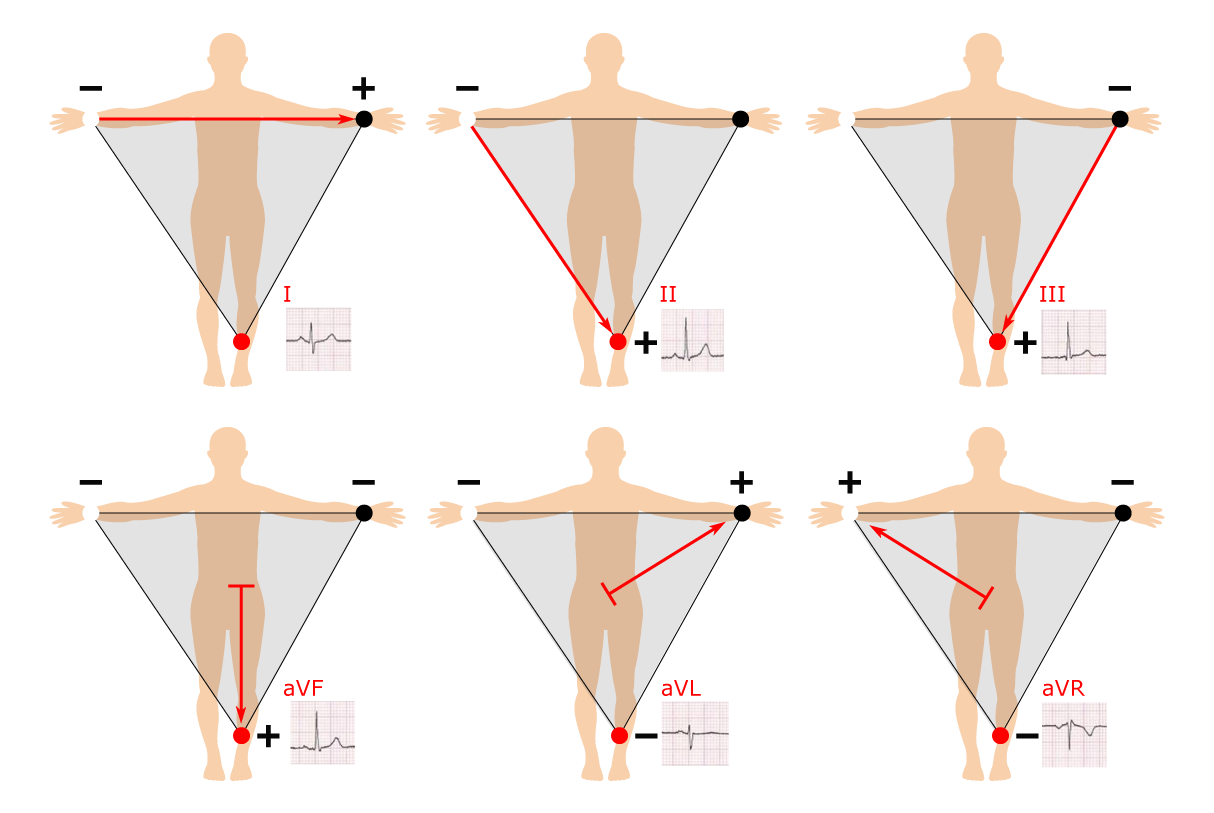
\includegraphics[scale=.2]{image/week1/chuyendaochi.png}
    \end{center}
    \caption{Chuyển đạo chi \cite{chuyendao}}
    \end{figure}
\end{center}
Tất cả 6 chuyển đạo: D1, D2, D3, aVR, aVL, aVF được gọi chung là các chuyển đạo ngoại biên vì đều có điện cực thăm dò đặt ở các chi. Chúng hỗ trợ cho nhau “dò xét” các rối loạn của dòng điện tim thể hiện ở bốn phía xung quanh quả tim trên mặt phẳng chắn (frontal plane).
\begin{center}
    \begin{figure}[htp]
    \begin{center}
    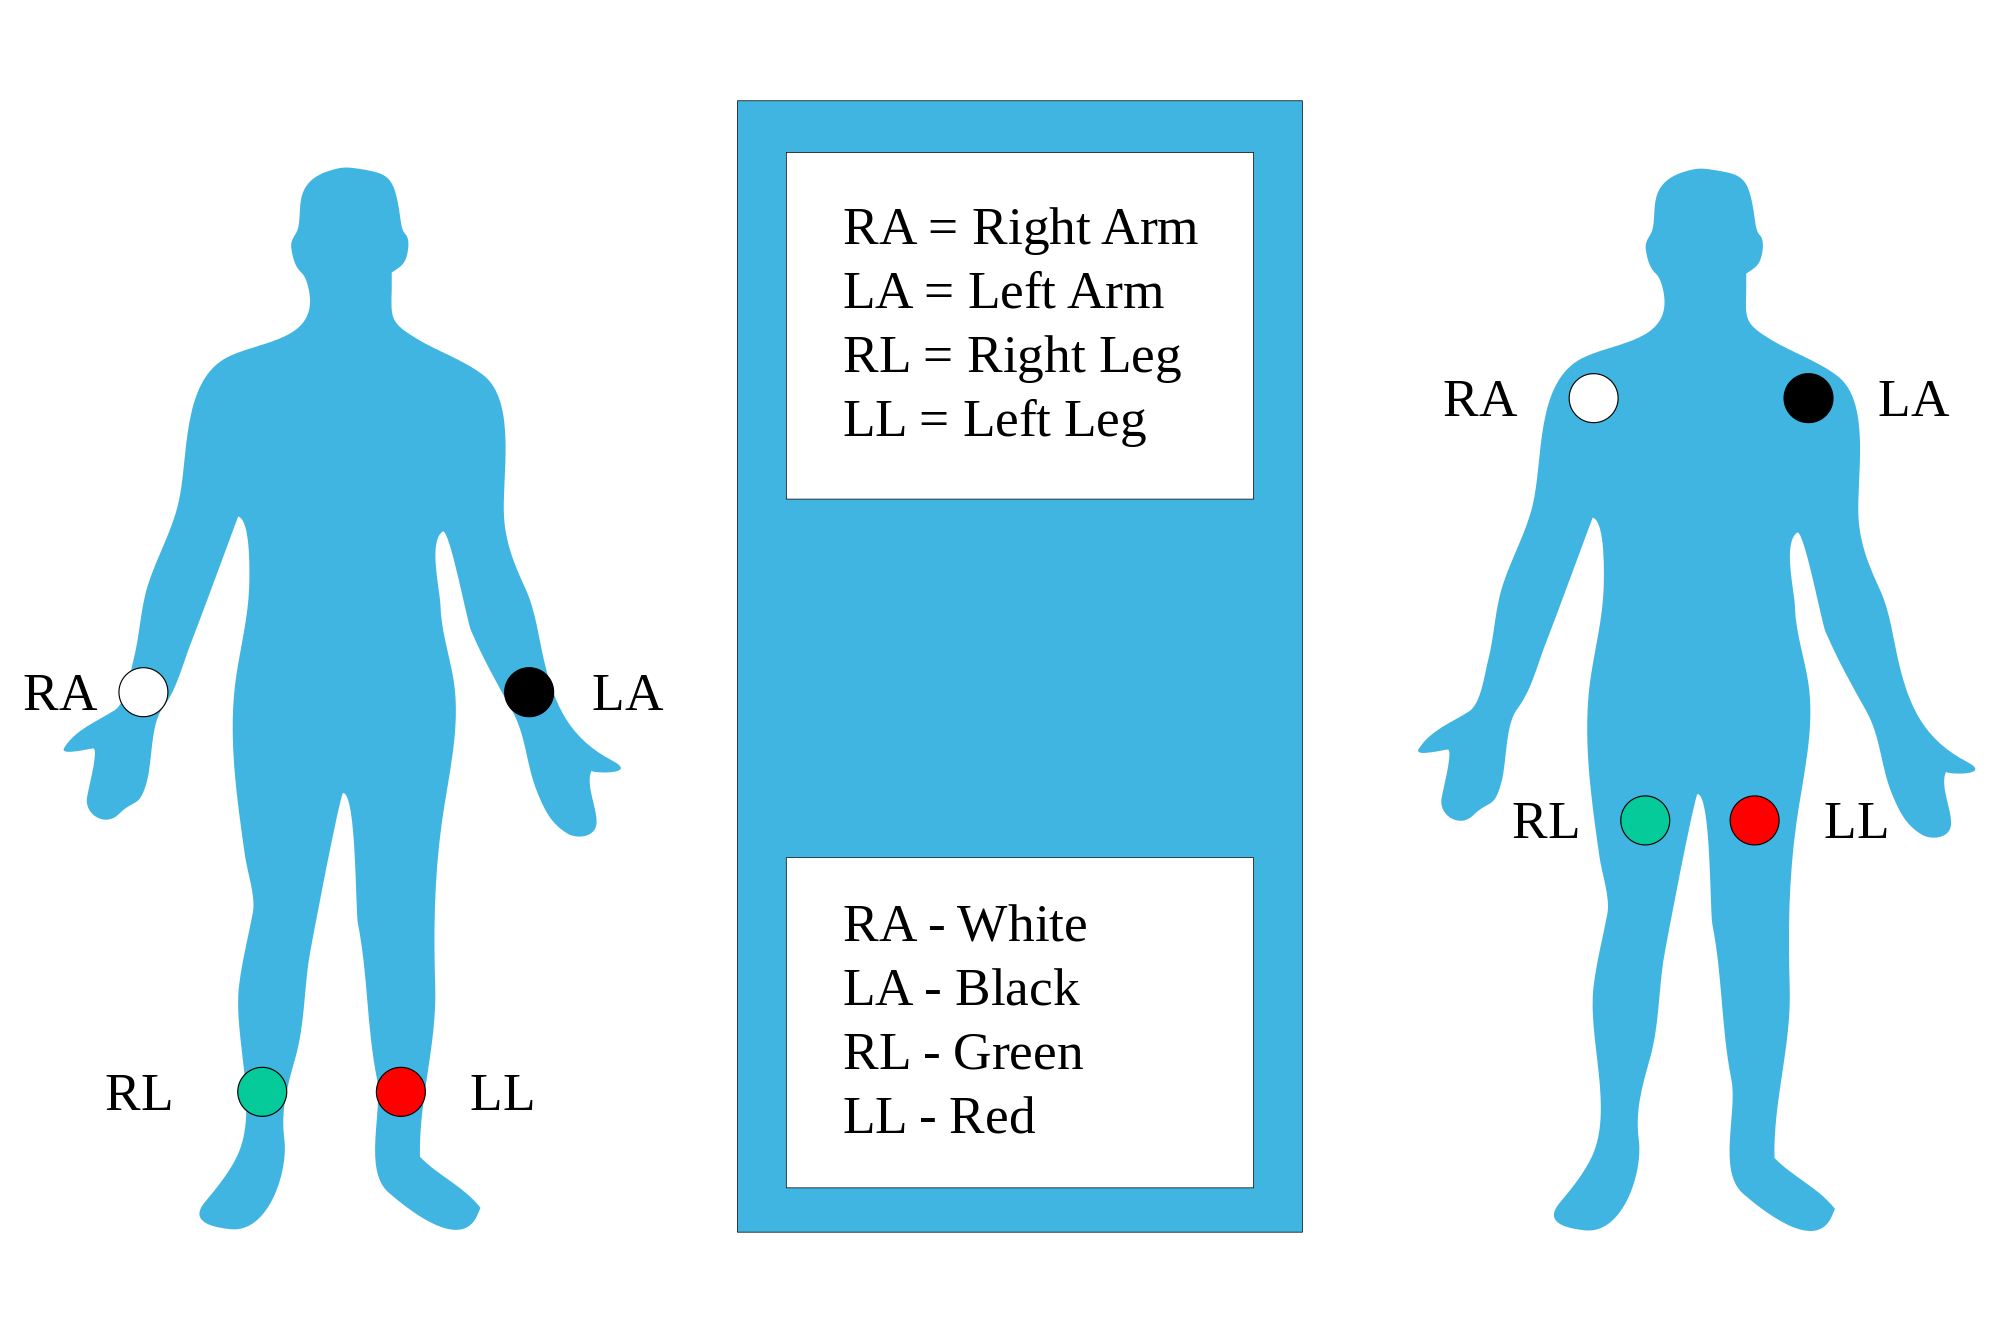
\includegraphics[scale=.12]{image/chapter1/2000px-Limb_leads.png}
    \end{center}
    \caption{Các vị trí đặt điện cực để đo ECG}
    \end{figure}
\end{center}

\subsubsection{Chuyển đạo trước tim:}
\begin{center}
    \begin{figure}[htp]
    \begin{center}
    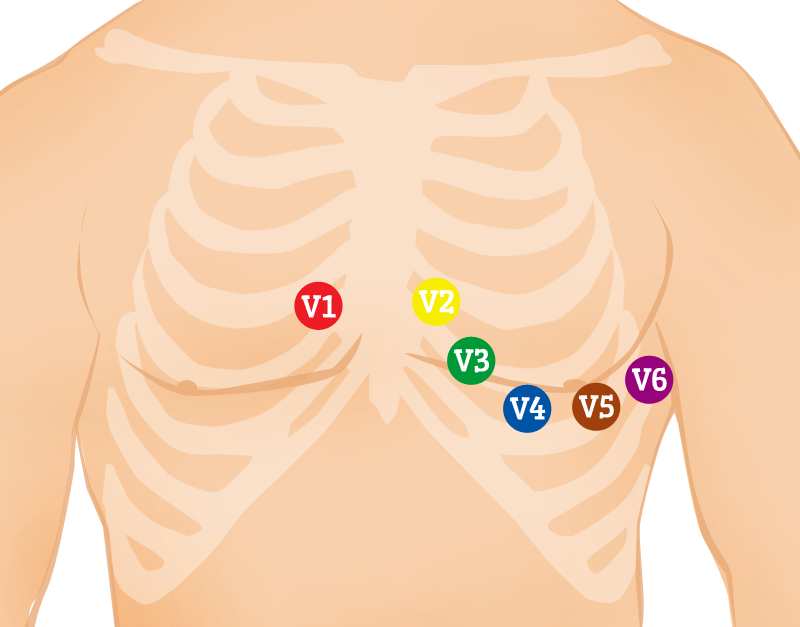
\includegraphics[scale=.25]{image/week1/chuyendaotruocnguc.png}
    \end{center}
    \caption{Chuyển đạo trước tim }
    \end{figure}
\end{center}
Người ta thường ghi đồng loạt cho bệnh nhân 6 chuyển đạo trước tim thông dụng nhất, kí hiệu bằng chữ V (voltage) kèm theo các chỉ số từ 1 đến 6.(V1, V2,…,V6).

\subsubsection{Một số chuyển đạo khác:}
V7, V8, V9(điện cực ở mé trái và sau lồng ngực dùng để thăm dò thất trái), V3R, V4R, V5R, V6R(điện cực ở mé phải lồng ngực dùng để nghiên cứu thất phải hay tim sang phải), chuyển đạo thực quản (Kí hiệu VOE), chuyển đạo trong buồng tim, điện đồ His.

\subsection{Đo điện tâm đồ}
\subsubsection{Đo điện tâm đồ truyền thống}
Định dạng chuẩn của một điện tâm đồ là điện tâm đồ được ghi lại trên một khổ giấy
.Để đánh giá thời gian dài hay ngắn và biên độ cao hay thấp của các làn sóng điện tâm đồ, người ta đinh chuẩn: 
\begin{itemize}
    \item Vận tốc 25mm/s thì mỗi ô 1mm có giá trị 0,04s.
    \item Theo chiều ngang 1 ô lớn tương ứng với 1000ms.
    \item Theo chiều dọc 1 ô lớn tương ứng 500mV.
\end{itemize}
\begin{center}
    \begin{figure}[htp]
    \begin{center}
    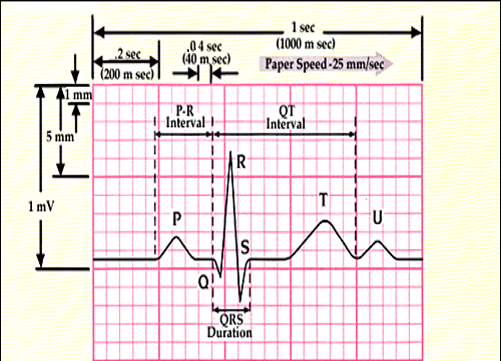
\includegraphics[scale=.6]{image/week1/new_ecg_paper.png}
    \end{center}
    \caption{Hình ảnh một chu kỳ sóng được đo theo kích thước khổ giấy, bác sĩ căn cứ vào ô trên giấy để phát hiện bất thường ở ECG \cite{ecggiay}}
    \end{figure}
\end{center}
\subsubsection{Đo điện tâm đồ bằng thiết bị di động thông minh (Apple Watch Series 4)}
Tính năng ECG hay còn gọi là đo điện tâm đồ đã chính thức có thể sử dụng trên Apple Watch Series 4 để phát hiện nhịp tim bất thường và chẩn đoán các bệnh tim nghiêm trọng.
\begin{center}
    \begin{figure}[htp]
    \begin{center}
    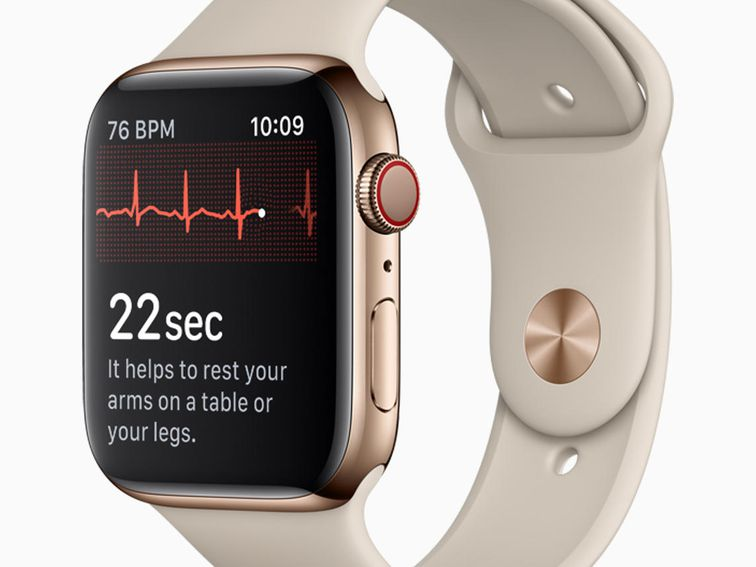
\includegraphics[scale=.3]{image/chapter1/apple-watch-series4-ecg-crown-09122018.jpg}
    \end{center}
    \caption{Apple Watch Series 4}
    \end{figure}
\end{center}
% \section{Đọc một điện tâm đồ}
% \subsection{Những bước phân tích trước khi đọc một điện tâm đồ}
% Điện tâm đồ (ECG) là một đường cong ghi lại các biến thiên của các điện lực do tim phát ra trong khi hoạt động co bóp.\cite{huongdanDTT}

% \begin{enumerate}
%     \item Trước khi đọc điện tâm đồ, phải nắm vững tuổi, giới tính, chẩn đoán lâm sàng của bệnh
%     nhân. Ngoài ra, còn nên biết thêm sơ lược bệnh án, hình ảnh X quang, các kết quả xét nghiệm khác và nhất là hai vấn đề sau đây:
%     \begin{itemize}
%         \item Khổ người bệnh nhân gầy béo, cao thấp ảnh hưởng rất nhiều đến tư thế tìm và biên độ sóng, nó ảnh hưởng nhiều đến chẩn đoán dày thất.
%         \item Có đang dùng thuốc trợ tim hay thuốc chống loạn nhịp dài ngày không? Nhất là digitan và quinidin… vì các thuốc này tác động rất nhiều đến hình dạng điện tâm đồ và dễ làm sai lạc chẩn đoán cơ bản.
%     \end{itemize}
%     \item Kiểm tra kỹ thuật ghi điện tâm đồ, phát hiện ghi sai, ảnh hưởng tạp, milivôn lấy đúng 1cm
%     hay không? Tốc độ ghi bao nhiêu? Nghĩa là các đường kẻ dọc cách nhau bao nhiêu phần trăm
%     giây
%     \item Nhịp tim: bước vào đọc điện tâm đồ trước hết bao giờ cũng phải xem nhịp xoang hay
%     không xoang? Có những rối loạn nhịp tim gì? Đừng bao giờ quên tính tần số tim. Nếu có blốc
%     nhĩ-thất thì phải tính riêng cả tần số nhĩ.
%     \item Trục điện tim với góc alpha, tư thế tim.
%     \item Hình dạng các sóng: đọc đồng thời ở cả 12 chuyển đạo thông dụng:
%     \begin{itemize}
%         \item Sóng P: chiều cao (biên độ), chiều rộng (thời gian), hình dạng (âm, dương, hai pha, móc).
%         \item Khoảng PQ dài bao nhiêu?
%         \item Phức bộ QRS: biên độ và thời gian chung và riêng của sóng Q, hình dạng (móc…).
%         \item Riêng với V1 và V5 thì tìm thêm thời gian xuất hiện nhánh nội điện.
%         \item Đoạn ST có chênh không?
%         \item Sóng T (và sóng U): dạng (dương, âm hay hai pha), biên độ.
%         \item Khoảng QT dài bao nhiêu?
%     \end{itemize}
%     \item Kết luận chẩn đoán: về tổn thương cơ tim và về rối loạn nhịp tim.
% \end{enumerate}

\chapter{Dữ liệu về điện tim}
\newpage

\section{Physionet}
\subsection{Thông tin về dataset}
Là một trang web truy cập miễn phí các bộ dữ liệu lớn về tín hiệu sinh lý được ghi lại (PhysioBank) và những phần mềm mã nguồn mở liên quan (PhysioToolkit).
\begin{center}
    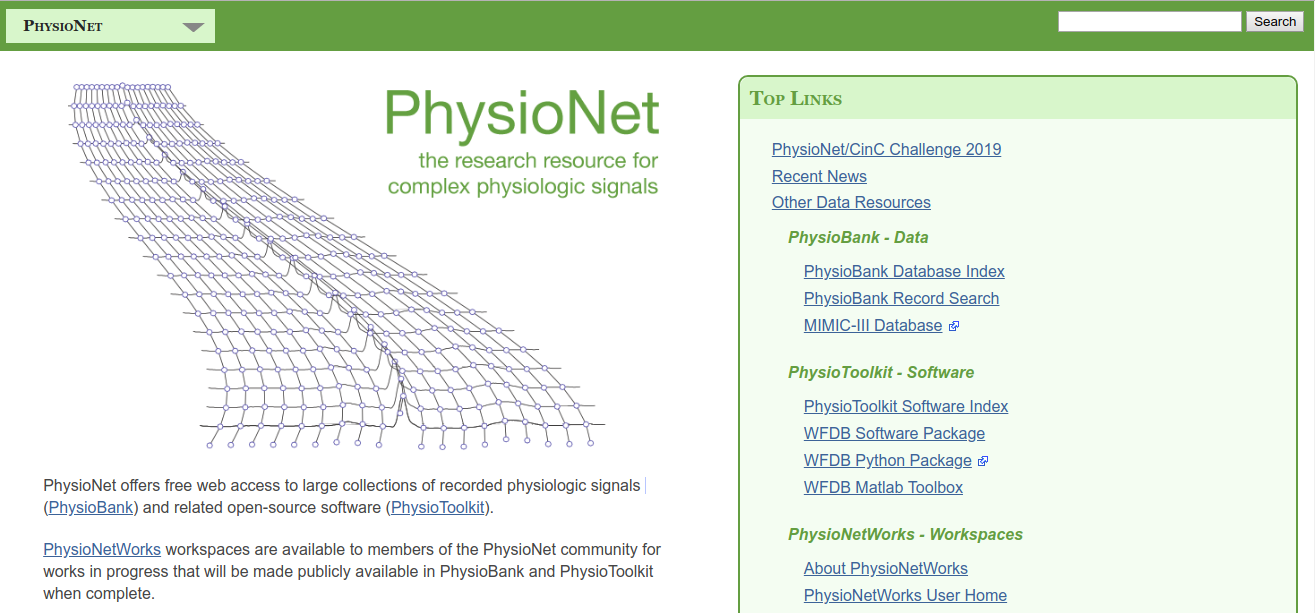
\includegraphics[scale=.3]{image/chapter3/Screenshot_from_2019-03-11_04-58-18.png}
    \begin{figure}[htp]
    \begin{center}
    \end{center}
    \caption{Trang Physionet}
    \end{figure}
\end{center}

\subsection{MIT-BIH Arrhythmia Database}
\textbf{Thông tin về database}
Đây là bộ dữ liệu nổi tiếng nhất, nhiều bài báo cũng như nghiên cứu dựa trên bộ dữ liệu này. Tập dữ liệu bao gồm 48 file. Mỗi file gồm: 1 file dat chứa dữ liệu, một file atr chứa chú thích, 1 file hea chứa header.
\begin{center}
    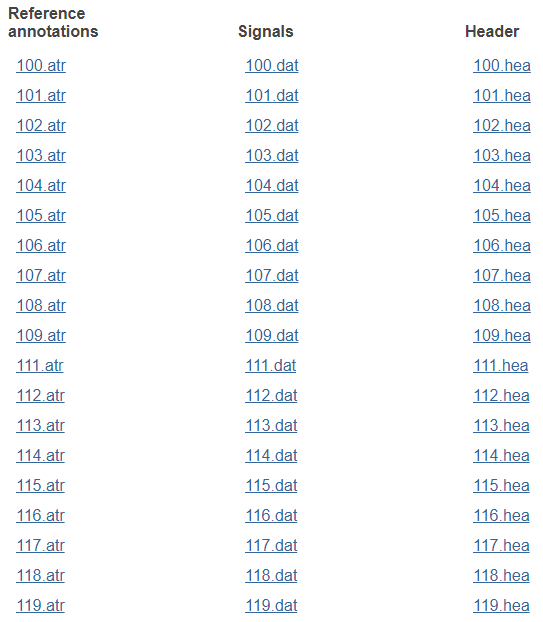
\includegraphics[scale=.4]{image/week3/mit.png}
    \begin{figure}[htp]
    \begin{center}
    \end{center}
    \caption{Dataset sample}
    \end{figure}
\end{center}
Phân tích và plot file 100.mat thành đồ thị.
\begin{center}
    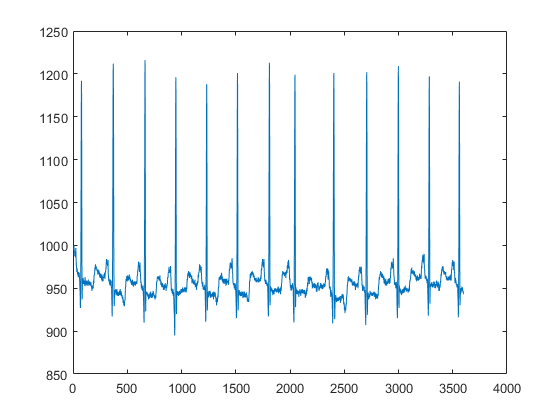
\includegraphics[scale=.8]{image/week4/100dat.png}
    \begin{figure}[htp]
    \begin{center}
    \end{center}
    \caption{100.mat sau khi plot thành đồ thị thể hiện hình dạng ECG}
    \end{figure}
\end{center}

\chapter{Những kiến thức nền tảng trong một mô hình phát hiện bất thường ở điện tâm đồ}
\newpage

\section{Kỹ thuật lọc nhiễu Butterworth}
Bộ lọc Butterworth là một loại bộ lọc xử lý tín hiệu được thiết kế để có đáp ứng tần số càng phẳng càng tốt trong băng thông. Nó cũng được gọi là một bộ lọc cường độ phẳng tối đa. Nó được mô tả lần đầu tiên vào năm 1930 bởi kỹ sư và nhà vật lý người Anh Stephen Butterworth trong bài báo của ông có tựa đề "Về lý thuyết của bộ khuếch đại bộ lọc".
\section{Kỹ thuật ngưỡng kích ứng thích hợp}

\section{Mạng Neural Hồi quy (RNN)}
\subsection{Giới thiệu}
Con người không bắt đầu suy nghĩ của họ từ đầu tại tất cả các thời điểm. Cũng như bạn đang đọc bài viết này, bạn hiểu mỗi chữ ở đây dựa vào từ bạn đã hiểu các chữ trước đó chứ không phải là đọc tới đâu ném hết đi tới đó, rồi lại bắt đầu suy nghĩ lại từ đầu tới chữ bạn đang đọc. Tức là tư duy đã có một bộ nhớ để lưu lại những gì diễn ra trước đó.\\
Tuy nhiên các mô hình mạng nơ-ron truyền thống thì không thể làm được việc đó, đó có thể coi là một khuyết điểm chính của mạng nơ-ron truyền thống. Ví dụ, bạn muốn phân loại các bối cảnh xảy ra ở tất cả các thời điểm trong một bộ phim, thì đúng là không rõ làm thế nào để có thể hiểu được một tình huống trong phim mà lại phụ thuộc vào các tình huống trước đó nếu sử dụng các mạng nơ-ron truyền thống.\\
Mạng nơ-ron hồi quy (Recurrent Neural Network) sinh ra để giải quyết vấn đề đó. Mạng này chứa các vòng lặp bên trong cho phép thông tin có thể lưu lại được.
\begin{center}
    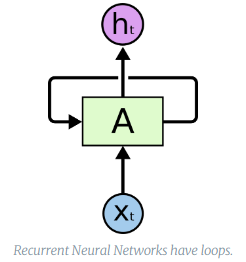
\includegraphics[scale=.5]{image/chapter6/RNN-node.png}
    \begin{figure}[htp]
    \begin{center}
    \end{center}
    \caption{một đoạn của mạng nơ-ron hồi quy A với đầu vào là $x_{n}$ và đầu ra là $h_{t}$. Một vòng lặp cho phép thông tin có thể được truyền từ bước này qua bước này qua bước khác của mạng nơ-ron. \cite{rnn-basic}}
    \end{figure}
\end{center}
Một mạng nơ-ron hồi quy có thể được coi là nhiều bản sao chép của cùng một mạng, trong đó mỗi đầu ra của mạng này là đầu vào của một mạng sao chép khác.\par
\begin{center}
    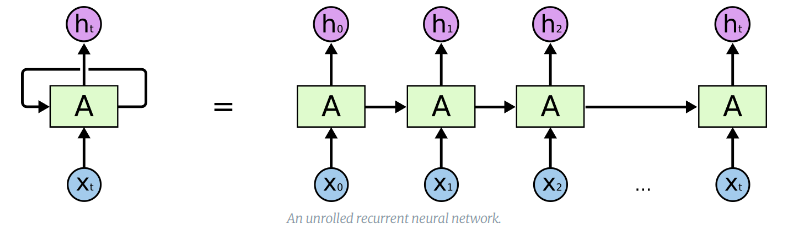
\includegraphics[scale=.5]{image/chapter6/RNN-ab.png}
    \begin{figure}[htp]
    \begin{center}
     
    \end{center}
    \caption{Chuỗi lặp lại các mạng này chính là phân giải của mạng nơ-ron hồi quy, các vòng lặp khiến chúng tạo thành một chuỗi danh sách các mạng sao chép nhau. \cite{rnn-basic}}
    \end{figure}
\end{center}
Một cách chi tiết hơn.
\begin{center}
    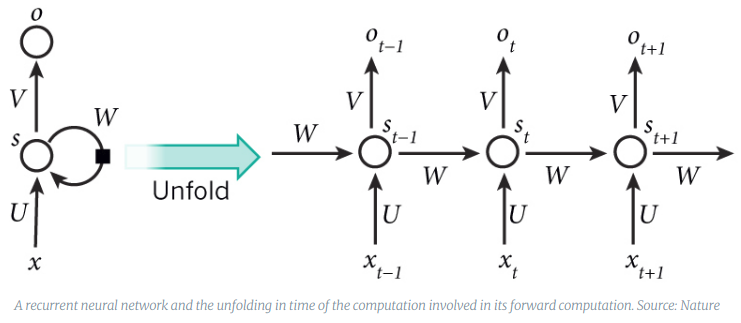
\includegraphics[scale=.4]{image/chapter6/rnn-detail.png}
    \begin{figure}[htp]
    \begin{center}
     
    \end{center}
    \caption{Chi tiết mạng RNN \cite{rnn-basic}}
    \end{figure}
\end{center}
\begin{itemize}
    \item $x_{t}$ là đầu vào tại bước t.
    \item $s_{t}$ là trạng thái ẩn tại bước t. Nó chính là bộ nhớ của mạng. $s_{t}$ được tính toán dựa trên cả các trạng thái ẩn phía trước và đầu vào tại bước đó: $s_{t} = f(Ux_{t}+Ws_{t-1})$. Hàm $f$ thường là một hàm phi tuyến như tang hyperbolic (tanh) hay Relu. Để làm phép toán cho phần tử ẩn đầu tiên ta cần khởi tạo thêm $s_{-1}$, thường giá trị khởi tạo được gắn bằng 0.
    \item $o_{t}$ là đầu ra tại bước t. Ví dụ, ta muốn dự đoán từ tiếp theo có thể xuất hiện trong câu thì $o_{t}$ chính là một vec-tơ xác xuất các từ trong danh sách từ vựng của ta: $o_{t} = softmax(Vs_{t})$. 
\end{itemize}


\subsection{Một số ứng dụng của RNN}
\begin{itemize}
    \item Nhận dạng giọng nói: Đưa vào một chuỗi các tín hiệu âm thanh, ta có thể dự đoán được chuỗi các đoạn ngữ âm đi kèm với xác xuất của chúng.
    \item Mô tả hình ảnh: Cùng với ConvNet, RNN được sử dụng để tự động tạo mô tả cho các ảnh chưa được gán nhãn. Sự kết hợp này đã đưa ra được các kết quả khá kinh ngạc. Ví dụ như các ảnh dưới đây, các mô tả sinh ra có mức độ chính xác và độ tường tận khá cao.
    \begin{center}
    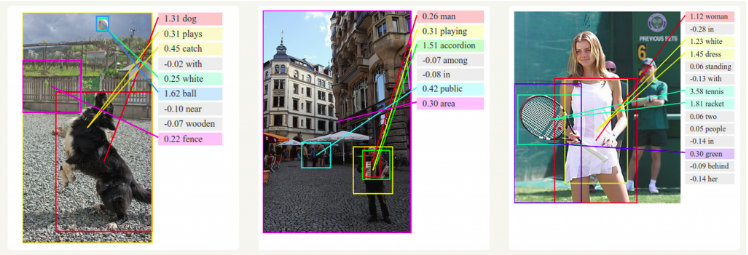
\includegraphics[scale=.4]{image/chapter6/RNN-application.png}
    \begin{figure}[htp]
    \begin{center}
     
    \end{center}
    \caption{Ứng dụng của RNN trong phân loại ảnh \cite{rnn-basic}}
    \end{figure}
    \end{center}
\end{itemize}


\subsection{RNN mở rộng}
\begin{itemize}
    \item RNN 2 chiều: Ở mô hình RNN 2 chiều (Bidirectional RNN), đầu ra tại bước t không những phụ thuộc vào các phần tử phía trước mà còn phụ thuộc cả vào các phần tử phía sau. Ví dụ, để dự đoán từ còn thiếu trong câu, thì việc xem xét cả phần trước và phần sau của câu là cần thiết. Vì vậy, ta có thể coi mô hình là việc chồng 2 mạng RNN ngược hướng nhau lên nhau. Lúc này đầu ra được tính toán dựa vào cả 2 trạng thái ẩn của 2 mạng RNN ngược hướng này.
    \begin{center}
    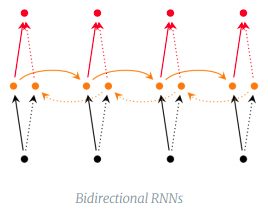
\includegraphics[scale=.5]{image/chapter6/RNN-2.png}
    \begin{figure}[htp]
    \begin{center}
     
    \end{center}
    \caption{RNN 2 chiều \cite{rnn-basic}}
    \end{figure}
    \end{center}
    \item RNN (2 chiều) sâu: RNN sâu (Deep (Bidirectional) RNN) cũng tương tự như RNN 2 chiều, nhưng khác nhau ở chỗ chúng chứa nhiều tầng ẩn ở mỗi bước. Trong thực tế, chúng giúp cho việc học ở mức độ cao hơn, tuy nhiên ta cũng cần phải có nhiều dữ liệu huấn luyện hơn.
    \begin{center}
    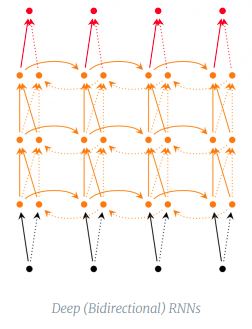
\includegraphics[scale=.3]{image/chapter6/RNN-4.png}
    \begin{figure}[htp]
    \begin{center}
     
    \end{center}
    \caption{RNN sâu \cite{rnn-basic}}
    \end{figure}
    \end{center}
\end{itemize}


\section{Mạng bộ nhớ ngắn dài (LSTM)}
\subsection{Vấn đề phụ thuộc xa}
Một điểm nổi bật của RNN chính là ý tưởng kết nối các thông tin phía trước để dự đoán cho hiện tại. Việc này tương tự như ta sử dụng các cảnh trước của bộ phim để hiểu được cảnh hiện thời. Nếu mà RNN có thể làm được việc đó thì chúng sẽ cực kì hữu dụng, tuy nhiên liệu chúng có thể làm được không? Câu trả lời là còn tùy.\\
Đôi lúc ta chỉ cần xem lại thông tin vừa có thôi là đủ để biết được tình huống hiện tại. Ví dụ, ta có câu: “các đám may trên bầu trời” thì ta chỉ cần đọc tới “các đám may trên bầu” là đủ biết được chữ tiếp theo là “trời” rồi. Trong tình huống này, khoảng cách tới thông tin có được cần để dự đoán là nhỏ, nên RNN hoàn toàn có thể học được.
\begin{center}
    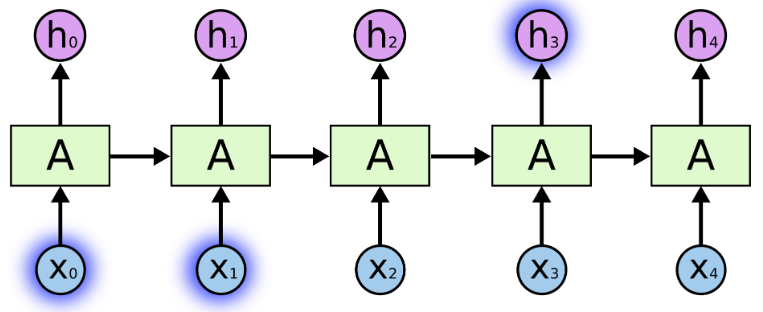
\includegraphics[scale=.3]{image/chapter6/ptx1.png}
    \begin{figure}[htp]
    \begin{center}
     
    \end{center}
    \end{figure}
\end{center}
Nhưng trong nhiều tình huống ta buộc phải sử dụng nhiều ngữ cảnh hơn để suy luận. Ví dụ, dự đoán chữ cuối cùng trong đoạn: “I grew up in France… I speak fluent French.”. Rõ ràng là các thông tin gần (”I speak fluent”) chỉ có phép ta biết được đằng sau nó sẽ là tên của một ngôn ngữ nào đó, còn không thể nào biết được đó là tiếng gì. Muốn biết là tiếng gì, thì ta cần phải có thêm ngữ cảnh “I grew up in France” nữa mới có thể suy luận được. Rõ ràng là khoảng cách thông tin lúc này có thể đã khá xa rồi.\\
Thật không may là với khoảng cách càng lớn dần thì RNN bắt đầu không thể nhớ và học được nữa.
\begin{center}
    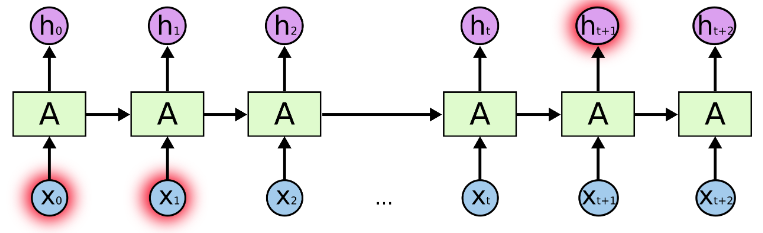
\includegraphics[scale=.3]{image/chapter6/ptx2.png}
    \begin{figure}[htp]
    \begin{center}
     
    \end{center}
    \end{figure}
\end{center}
Về mặt lý thuyết, rõ ràng là RNN có khả năng xử lý các phụ thuộc xa (long-term dependencies). Chúng ta có thể xem xét và cài đặt các tham số sao cho khéo là có thể giải quyết được vấn đề này. Tuy nhiên, đáng tiếc trong thực tế RNN có vẻ không thể học được các tham số đó. Vấn đề này đã được khám phá khá sâu bởi Hochreiter (1991) [tiếng Đức] và Bengio, et al. (1994), trong các bài báo của mình, họ đã tìm được nhưng lý do căn bản để giải thích tại sao RNN không thể học được.


\subsection{Mạng LSTM}
Mạng bộ nhớ dài-ngắn (Long Short Term Memory networks), thường được gọi là LSTM - là một dạng đặc biệt của RNN, nó có khả năng học được các phụ thuộc xa. LSTM được giới thiệu bởi Hochreiter và Schmidhuber (1997), và sau đó đã được cải tiến và phổ biến bởi rất nhiều người trong ngành. Chúng hoạt động cực kì hiệu quả trên nhiều bài toán khác nhau nên dần đã trở nên phổ biến như hiện nay.\\
LSTM được thiết kế để tránh được vấn đề phụ thuộc xa (long-term dependency). Việc nhớ thông tin trong suốt thời gian dài là đặc tính mặc định của chúng, chứ ta không cần phải huấn luyện nó để có thể nhớ được. Tức là ngay nội tại của nó đã có thể ghi nhớ được mà không cần bất kì can thiệp nào.\\
Mọi mạng hồi quy đều có dạng là một chuỗi các mô-đun lặp đi lặp lại của mạng nơ-ron. Với mạng RNN chuẩn, các mô-dun này có cấu trúc rất đơn giản, thường là một tầng $tanh$
\begin{center}
    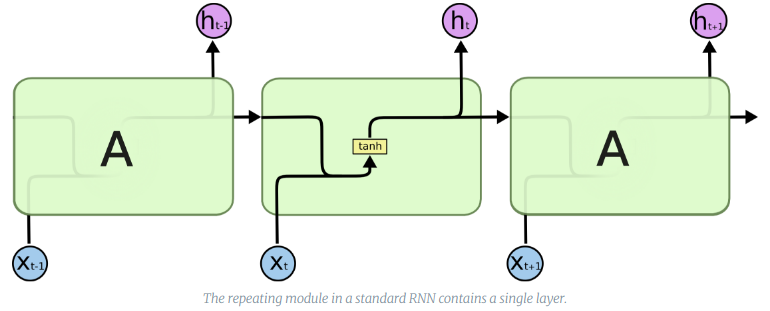
\includegraphics[scale=.3]{image/chapter6/lstm1.png}
    \begin{figure}[htp]
    \begin{center}
    \end{center}
    \end{figure}
\end{center}
LSTM cũng có kiến trúc dạng chuỗi như vậy, nhưng các mô-đun trong nó có cấu trúc khác với mạng RNN chuẩn. Thay vì chỉ có một tầng mạng nơ-ron, chúng có tới 4 tầng tương tác với nhau một cách rất đặc biệt.
\begin{center}
    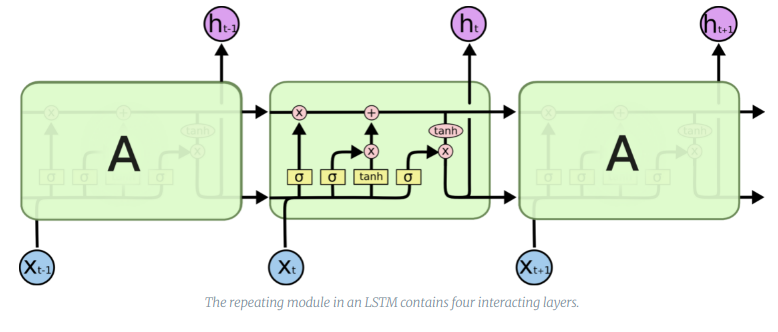
\includegraphics[scale=.3]{image/chapter6/lstm2.png}
    \begin{figure}[htp]
    \begin{center}
     
    \end{center}
    \end{figure}
\end{center}
Giờ thì đừng hoang mang về chi tiết bên trong chúng ngay, chúng ta sẽ khám phá chúng chi tiết chúng ở bước sau. Điều bạn cần làm bây giờ là làm hãy làm quen với các kí hiệu mà ta sẽ sử dụng ở dưới đây:
\begin{center}
    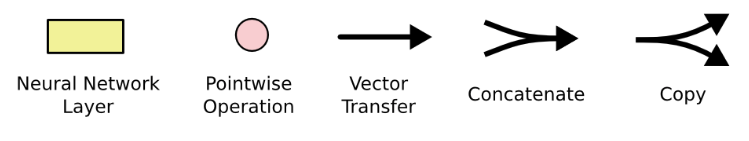
\includegraphics[scale=.3]{image/chapter6/lstm3.png}
    \begin{figure}[htp]
    \begin{center}
     
    \end{center}
    \end{figure}
\end{center}
Ở sơ đồ trên, mỗi một đường mang một véc-tơ từ đầu ra của một nút tới đầu vào của một nút khác. Các hình trong màu hồng biểu diễn các phép toán như phép cộng véc-tơ chẳng hạn, còn các ô màu vàng được sử dụng để học trong các từng mạng nơ-ron. Các đường hợp nhau kí hiệu việc kết hợp, còn các đường rẽ nhánh ám chỉ nội dung của nó được sao chép và chuyển tới các nơi khác nhau.


\subsection{Ý tưởng cốt lõi của LSTM}
Chìa khóa của LSTM là trạng thái tế bào (cell state) - chính đường chạy thông ngang phía trên của sơ đồ hình vẽ.\par
Trạng thái tế bào là một dạng giống như băng truyền. Nó chạy xuyên suốt tất cả các mắt xích (các nút mạng) và chỉ tương tác tuyến tính đôi chút. Vì vậy mà các thông tin có thể dễ dàng truyền đi thông suốt mà không sợ bị thay đổi.
\begin{center}
    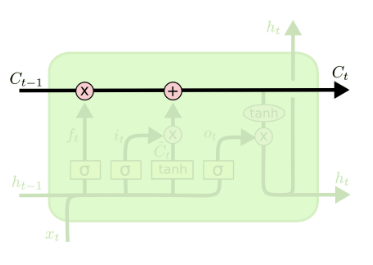
\includegraphics[scale=.5]{image/chapter6/yn1.png}
    \begin{figure}[htp]
    \begin{center}
     
    \end{center}
    \end{figure}
\end{center}
LSTM có khả năng bỏ đi hoặc thêm vào các thông tin cần thiết cho trạng thái tế báo, chúng được điều chỉnh cẩn thận bởi các nhóm được gọi là cổng (gate).\par
Các cổng là nơi sàng lọc thông tin đi qua nó, chúng được kết hợp bởi một tầng mạng sigmoid và một phép nhân.
\begin{center}
    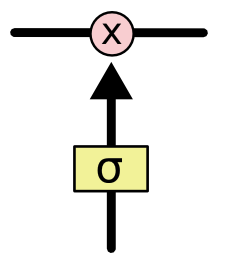
\includegraphics[scale=.3]{image/chapter6/yn2.png}
    \begin{figure}[htp]
    \begin{center}
     
    \end{center}
    \end{figure}
\end{center}
Tầng sigmoid sẽ cho đầu ra là một số trong khoản [0,1], mô tả có bao nhiêu thông tin có thể được thông qua. Khi đầu ra là 0 thì có nghĩa là không cho thông tin nào qua cả, còn khi là 1 thì có nghĩa là cho tất cả các thông tin đi qua nó.\\
Một LSTM gồm có 3 cổng như vậy để duy trì và điều hành trạng thái của tế bào.
\subsection{Bên trong LSTM}
Bước đầu tiên của LSTM là quyết định xem thông tin nào cần bỏ đi từ trạng thái tế bào. Quyết định này được đưa ra bởi tầng sigmoid - gọi là “tầng cổng quên” (forget gate layer). Nó sẽ lấy đầu vào là $h_{t-1}$ và $x_{t}$ rồi đưa ra kết quả là một số trong khoảng [0,1] cho mỗi số trong trạng thái tế bào $C_{t-1}$ Đẩu ra là 1 1 thể hiện rằng nó giữ toàn bộ thông tin lại, còn 0 chỉ rằng toàn bộ thông tin sẽ bị bỏ đi.\\
Quay trở lại với ví dụ mô hình ngôn ngữ dự đoán từ tiếp theo dựa trên tất cả các từ trước đó, với những bài toán như vậy, thì trạng thái tế bào có thể sẽ mang thông tin về giới tính của một nhân vật nào đó giúp ta sử dụng được đại từ nhân xưng chuẩn xác. Tuy nhiên, khi đề cập tới một người khác thì ta sẽ không muốn nhớ tới giới tính của nhân vật nữa, vì nó không còn tác dụng gì với chủ thế mới này.
\begin{center}
    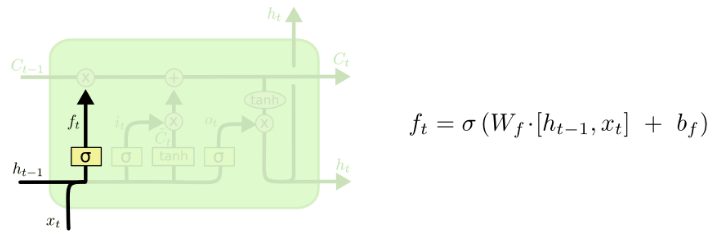
\includegraphics[scale=.5]{image/chapter6/bt1.png}
    \begin{figure}[htp]
    \begin{center}
     
    \end{center}
    \end{figure}
\end{center}
Bước tiếp theo là quyết định xem thông tin mới nào ta sẽ lưu vào trạng thái tế bào. Việc này gồm 2 phần. Đầu tiên là sử dụng một tầng sigmoid được gọi là “tầng cổng vào” (input gate layer) để quyết định giá trị nào ta sẽ cập nhập. Tiếp theo là một tầng $tanh$ tạo ra một véc-tơ cho giá trị mới $\widetilde{C}_{t}$ nhằm thêm vào cho trạng thái. Trong bước tiếp theo, ta sẽ kết hợp 2 giá trị đó lại để tạo ra một cập nhập cho trạng thái.\\
Chẳng hạn với ví dụ mô hình ngôn ngữ của ta, ta sẽ muốn thêm giới tính của nhân vật mới này vào trạng thái tế bào và thay thế giới tính của nhân vật trước đó.
\begin{center}
    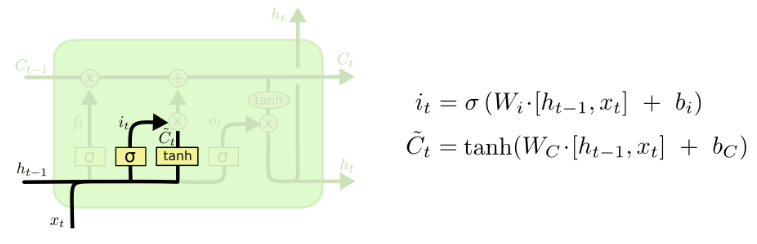
\includegraphics[scale=.5]{image/chapter6/bt2.png}
    \begin{figure}[htp]
    \begin{center}
     
    \end{center}
    \end{figure}
\end{center}
Giờ là lúc cập nhập trạng thái tế bào cũ $C_{t-1}$ thành trạng thái mới $C_{t}$ Ở các bước trước đó đã quyết định những việc cần làm, nên giờ ta chỉ cần thực hiện là xong.\\
Ta sẽ nhân trạng thái cũ với $f_{t}$ để bỏ đi những thông tin ta quyết định quên lúc trước. Sau đó cộng thêm $i_{t} * \widetilde{C}_{t}$. Trạng thái mơi thu được này phụ thuộc vào việc ta quyết định cập nhập mỗi giá trị trạng thái ra sao.\\
Với bài toàn mô hình ngôn ngữ, chính là việc ta bỏ đi thông tin về giới tính của nhân vật cũ, và thêm thông tin về giới tính của nhân vật mới như ta đã quyết định ở các bước trước đó.
\begin{center}
    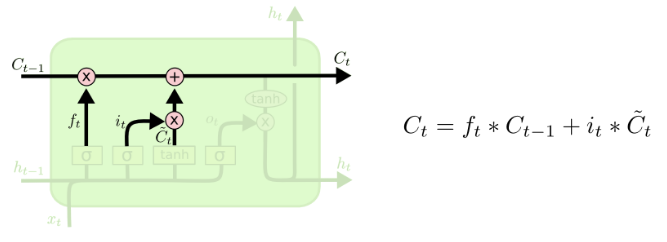
\includegraphics[scale=.5]{image/chapter6/bt3.png}
    \begin{figure}[htp]
    \begin{center}
     
    \end{center}
    \end{figure}
\end{center}
Cuối cùng, ta cần quyết định xem ta muốn đầu ra là gì. Giá trị đầu ra sẽ dựa vào trạng thái tế bào, nhưng sẽ được tiếp tục sàng lọc. Đầu tiên, ta chạy một tầng sigmoid để quyết định phần nào của trạng thái tế bào ta muốn xuất ra. Sau đó, ta đưa nó trạng thái tế bảo qua một hàm tanh để co giá trị nó về khoảng [-1, 1], và nhân nó với đầu ra của cổng sigmoid để được giá trị đầu ra ta mong muốn.\par
Với ví dụ về mô hình ngôn ngữ, chỉ cần xem chủ thể mà ta có thể đưa ra thông tin về một trạng từ đi sau đó. Ví dụ, nếu đầu ra của chủ thể là số ít hoặc số nhiều thì ta có thể biết được dạng của trạng từ đi theo sau nó phải như thế nào.
\begin{center}
    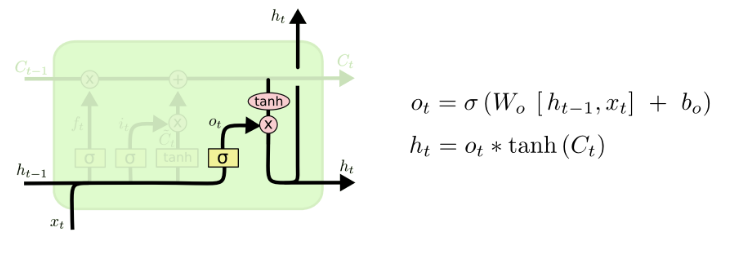
\includegraphics[scale=.5]{image/chapter6/bt4.png}
    \begin{figure}[htp]
    \begin{center}
     
    \end{center}
    \end{figure}
\end{center}


\subsection{Các biến thể của bộ nhớ dài hạn}
Những thứ ta vừa mô tả ở trên là một LSTM khá bình thường. Nhưng không phải tất cả các LTSM đều giống như vậy. Thực tế, các bài báo về LTSM đều sử dụng một phiên bản hơi khác so với mô hình LTSM chuẩn. Sự khác nhau không lớn, nhưng chúng giúp giải quyết phần nào đó trong cấu trúc của LTSM.\\
Một dạng LTSM phổ biến được giới thiệu bởi Gers và Schmidhuber (2000) được thêm các đường kết nối “peephole connections”, làm cho các tầng cổng nhận được giá trị đầu vào là trạng thái tế bào.
\begin{center}
    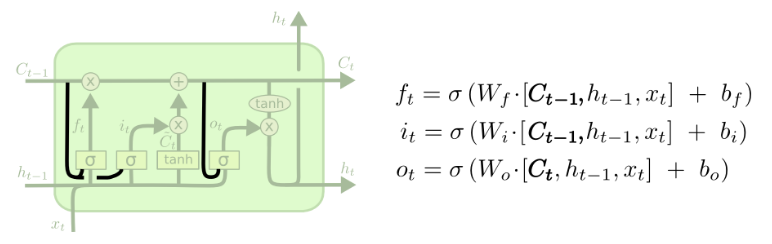
\includegraphics[scale=.5]{image/chapter6/bth1.png}
    \begin{figure}[htp]
    \begin{center}
     
    \end{center}
    \caption{Hình trên mô tả các đường được thêm vào mọi cổng, nhưng cũng có những bài báo chỉ thêm cho một vài cổng mà thôi.}
    \end{figure}
\end{center}
Một biến thể khác là nối 2 cổng loại trừ và đầu vào với nhau. Thay vì phân tách các quyết định thông tin loại trừ và thông tin mới thêm vào, ta sẽ quyết định chúng cùng với nhau luôn. Ta chỉ bỏ đi thông tin khi mà ta thay thế nó bằng thông tin mới đưa vào. Ta chỉ đưa thông tin mới vào khi ta bỏ thông tin cũ nào đó đi.
\begin{center}
    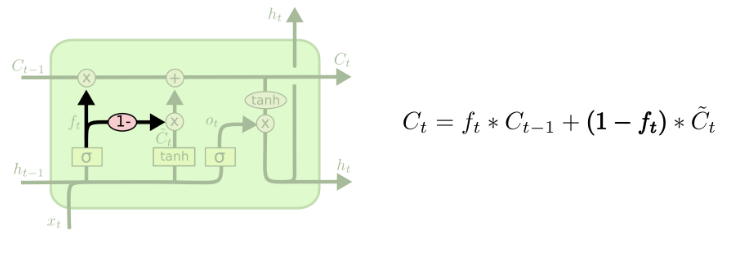
\includegraphics[scale=.5]{image/chapter6/bth2.png}
    \begin{figure}[htp]
    \begin{center}
     
    \end{center}
    \end{figure}
\end{center}
Một biến thể khá thú vị khác của LSTM là Gated Recurrent Unit, hay GRU được giới thiệu bởi Cho, et al. (2014). Nó kết hợp các cổng loại trừ và đầu vào thành một cổng “cổng cập nhập” (update gate). Nó cũng hợp trạng thái tế bào và trạng thái ẩn với nhau tạo ra một thay đổi khác. Kết quả là mô hình của ta sẽ đơn giản hơn mô hình LSTM chuẩn và ngày càng trở nên phổ biến.
\begin{center}
    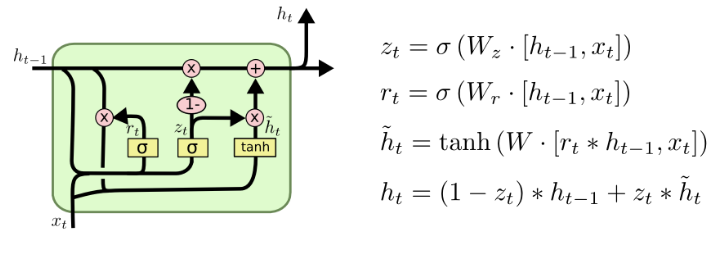
\includegraphics[scale=.5]{image/chapter6/bth3.png}
    \begin{figure}[htp]
    \begin{center}
     
    \end{center}
    \end{figure}
\end{center}
Trên đây chỉ là một vài biến thế được chú ý nhiều nhất thôi, thực tế có rất nhiều các biến thể khác nhau của LSTM như Depth Gated RNNs của Yao, et al. (2015). Cũng có những biến thể mà chiến lực xử lý phụ thuộc xa hoàn toàn khác như Clockwork RNNs của Koutnik, et al. (2014).\\
Nếu bạn muốn tìm hiểu xem biến thể nào là tốt nhất và chúng khác nhau thế nào, thì có thể đọc bài so sánh khá hay này của Greff, et al. (2015). Ngoài ra thì Jozefowicz, et al. (2015) thậm chí còn thử hàng chục nghìn kiến trúc RNN khác nhau và tìm ra một vài mô hình hoạt động tốt hơn cả LSTM ở một số bài toán.


\section{Kết luận}
RNN đặc biệt là LSTM được sử dụng nhiều trong những bài toán về chuỗi dữ liệu: mô hình ngôn ngữ, nhận dạng giọng nói,... Theo bài báo của Shraddha Singh và nhóm nghiên cứu mạng LSTM đem lại kết quả tốt nhất trong số 3 biến thể của RNN trong phân loại ECG-phát hiện đoạn run nhĩ RNN-acc:85.4\%, GRU-acc:82.5\%, LSTM-acc: 88.1\% \cite{ketluanlstm}.

\chapter{Mô hình phân loại điện tâm đồ }
\newpage

\section{Sơ đồ hệ thống phân loại điện tâm đồ}
\begin{center}
    
\includegraphics[scale=.5]{image/chapter5/system.png}
    \begin{figure}[htp]
    \begin{center}
    \end{center}
    \caption{Sơ đồ hệ thống phân loại điện tâm đồ}
    \end{figure}
\end{center}

\section{Tiền xử lý dữ liệu}
Tín hiệu điện tâm đồ khi được thu nhận từ các thiết bị đo ban đầu có khả năng rất cao bị nhiễu do nhiều yếu tố khác nhau, như nhiễu do ảnh hưởng từ cơ bắp, nhiễu sinh ra từ các thiết bị điện tử, nhiễu từ các điện cực của thiết bị đo điện tâm đồ, power line interference, baseline wander,… Nhiễu có tác động rất lớn đến chất lượng của việc trích xuất đặc trưng và do đó ảnh hưởng đến kết quả bài toán phân loại (việc trích xuất đặc trưng từ tín hiệu điện tâm đồ có thể không chính xác và do đó có thể dẫn đến kết quả phân loại, chẩn đoán bị sai). Vì vậy, tín hiệu điện tâm đồ được thu nhận lúc ban đầu cần phải được khử nhiễu trước khi được thực hiện các bước trích xuất đặc trưng và phân loại. Giải pháp cho việc khử nhiễu đó là lọc nhiễu Butterworth bậc 2 gồm high pass, low pass.
\begin{center}
         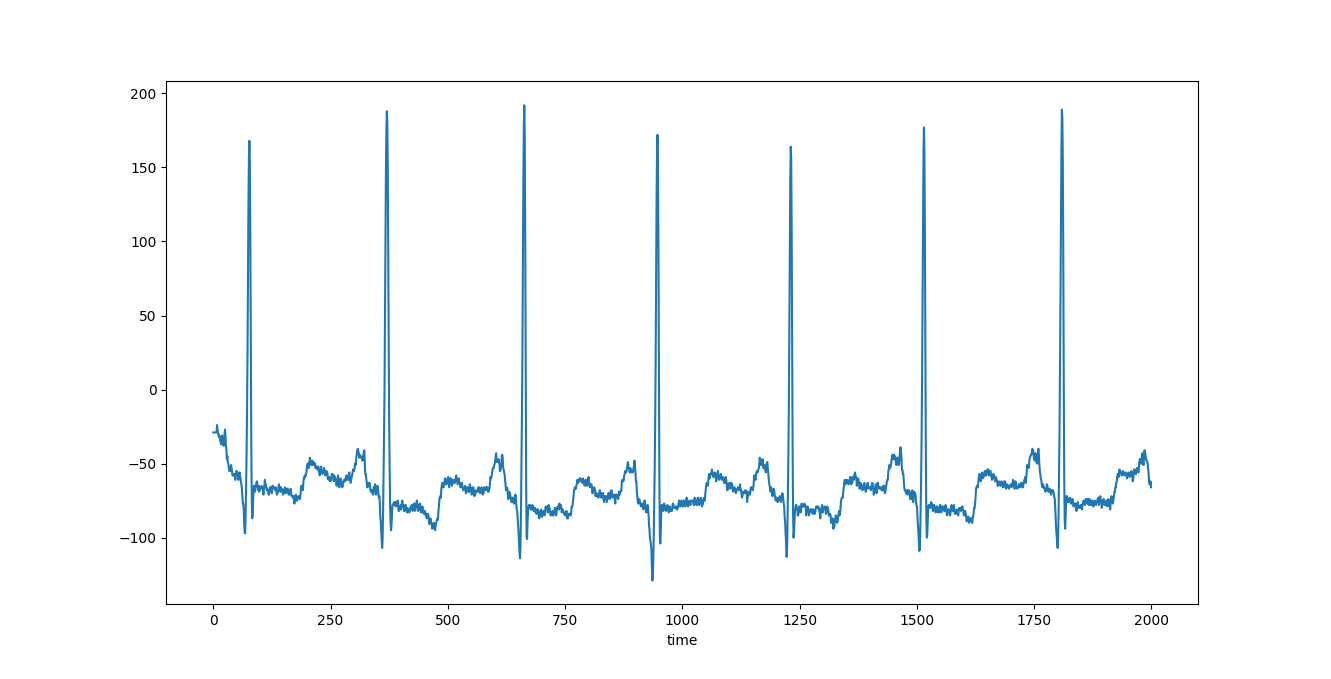
\includegraphics[width=1.\linewidth]{image/chapter5/noise.png}
         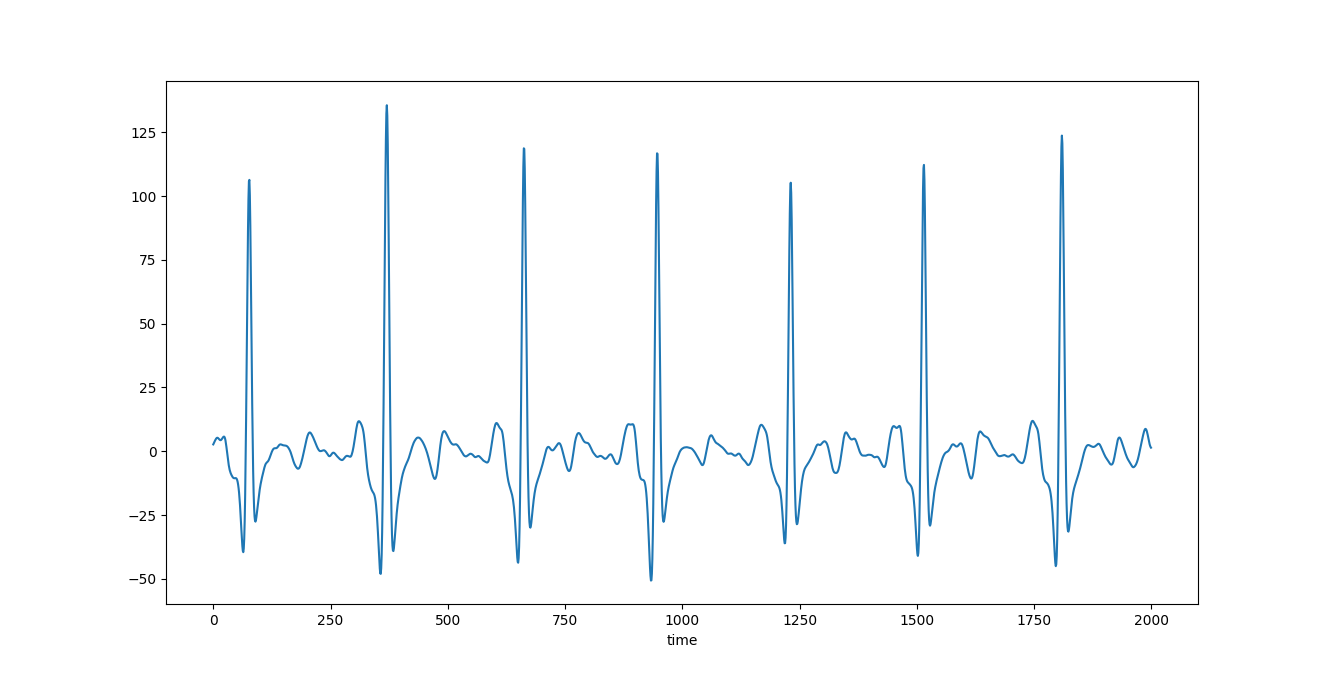
\includegraphics[width=1.\linewidth]{image/chapter5/hlp.png}
    \begin{figure}[!htb]
       \caption{Dữ liệu trước và sau khi lọc nhiễu}
    \end{figure}
\end{center}

\section{Trích xuất đặc trưng}
Dữ liệu sau khi xử lý tiền dữ liệu sẽ được trích xuất đặc trưng bằng kỹ thuật ngưỡng thích ứng kết hợp được đề xuất bới Christov. Những điểm R trong dữ liệu sẽ được đánh nhãn R
\begin{center}
    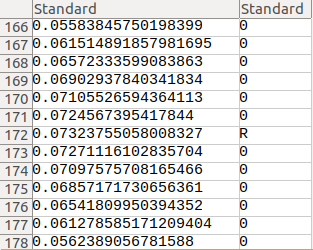
\includegraphics[scale=.5]{image/model/fx_rr.png}
    \begin{figure}[htp]
    \begin{center}
    \end{center}
    \caption{Dữ liệu csv đã được đánh dấu đoạn RR}
    \end{figure}
\end{center}
\begin{center}
    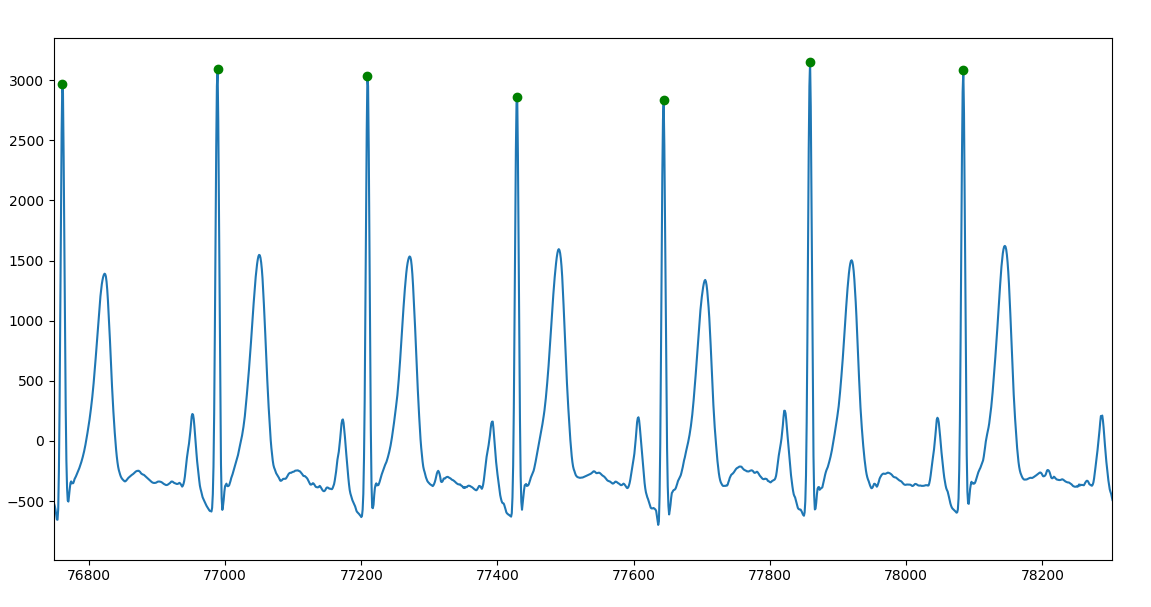
\includegraphics[scale=.4]{image/chapter5/R_detect.png}
    \begin{figure}[htp]
    \begin{center}
    \end{center}
    \caption{Hình ảnh đỉnh R được đánh dấu}
    \end{figure}
\end{center}

\section{Chuẩn hóa đặc trưng độ dài và biên độ khoảng R-R }
Một trong những bước đặc biệt và có ảnh hưởng rất lớn đến chất lượng phân loại tín hiệu điện tâm đồ trong nghiên cứu này là việc chuẩn hóa hình dạng (shape normalization) cho đặc trưng khoảng R-R. Do đặc điểm sinh lý của tim mà các khoảng R-R thường có độ dài khác nhau (nhịp đập của tim thường không bất biến mà sẽ có một sự chênh lệch nhất định). Ở người bình thường, không mắc các bệnh lý về tim mạch, khoảng R-R sẽ dao động trong khoảng 600 – 1200 ms \cite{64} . Sự chênh lệch này tuy không lớn về mặt sinh học nhưng sẽ ảnh hưởng rất lớn đến chất lượng của bài toán phân loại tín hiệu điện tâm đồ. Chỉ một sự thay đổi nhỏ (thậm chí rất nhỏ) về hình dạng khoảng R-R, ví dụ giữa hai đỉnh R có chênh lệch một khoảng nhỏ (ví dụ: 0.01 s), sẽ cho ra một dữ liệu huấn luyện hoàn toàn mới cho bài toán phân loại điện tâm đồ và càng nhiều khoảng R-R có hình dạng dài ngắn khác nhau thì tập dữ liệu huấn luyện được sinh ra sẽ vô cùng lớn. Nếu sự không đồng nhất về mặt hình dạng của các khoảng R-R này không được giải quyết hiệu quả thì việc phân loại những tín hiệu điện tâm đồ mới, không có trong tập dữ liệu huấn luyện, sẽ gặp khó khăn và có thể dẫn đến kết quả phân loại, chẩn đoán không còn chính xác (trường hợp này được gọi là overfit – mô hình phân loại chỉ đáp ứng tốt với dữ liệu huấn luyện mà không còn đáp ứng tốt với dữ liệu kiểm thử hoàn toàn mới). Đó là lý do vì sao các khoảng R-R cần phải được chuẩn hóa về một hình dạng nhất định. Massagram và nhóm nghiên cứu \cite{67}, Bhola và nhóm nghiên cứu đều cho rằng 880 – 900 ms là khoảng thời gian phổ biến nhất của khoảng R-R \cite{68}. Do đó, toàn bộ khoảng R-R trong nghiên cứu này sẽ được chuẩn hóa về khoảng thời gian đồng nhất 900 ms bằng phương pháp nội suy tuyến tính (linear interpolation). Hình dạng của khoảng R-R sau khi đã được chuẩn hóa đồng nhất về cùng một khoảng nhất định sẽ gần như không sai lệch quá nhiều so với khoảng R-R ban đầu. Điều này đồng nghĩa với việc mỗi đoạn R-R sẽ có 324 samples dữ liệu.\\
Dữ liệu sau khi chuẩn hóa về mặt thời gian sẽ được chuẩn hóa tiếp theo chiều cao sóng để đưa về khoảng [0,1] để dể dàng cho việc phân loại.

\section{Phân loại tín hiệu điện tâm đồ}
Mô hìn phân loại tín hiệu điện tâm đồ gồm sự kết hợp giữa mạng LSTM và tâng Fully-connected. Trong đó:
\begin{itemize}
    \item Mạng LSTM ở phần đầu của mô hình có chức năng học những đặc trưng tín hiệu điện tâm đồ có dạng Sequence-to-Sequence (Seq2Seq)
    \item Tầng Fully-Connected ở tầng cuối cùng của mô hình có chức năng phân loại dữ liệu đã được huấn luyện ở mạng LSTM trước đó dựa trên 2 nhãn (label) được cung cấp trước đó là “bình thường” (0) và “bất thường” (1)
\end{itemize}
Các tham số của mô hình phân loại:
\begin{itemize}
    \item Tham số tốc độ học (learning rate) là 0.001, giá trị này ảnh hưởng đến tốc độ hội tụ của quá trình huấn luyện.
    \item Số neuron đầu vào là 128, kích thước thu được khi qua mô hình autoencoder.
    \item Số lượng tầng Fully Connected: 2. Số lượng neuron tầng FC1: 20, số lượng neuron tâng FC2: 20 (có kết hợp kỹ thuật dropout).
    \item Hàm biến đổi: softmax.
    \item Hàm lỗi: Mean Square Error.
    \item Sô lớp phân loại tương ứng với 2 nhãn bình thường (0) và bất thường (1)
    \item Các kỹ thuật tránh overfit: Regularization L2, Dropout, khởi tạo trọng số kiểu Xavier.
    \item Phương pháp tối ưu hóa hàm lỗi: bộ tối ưu SGD.
    \item Số lần tính toán (epoch): 2200.
\end{itemize}

\section{Kết quả, Đánh giá và Trở ngại}
\subsection{Thu thập dữ liệu}
Dữ liệu chủ yếu trong nghiên cứu lần này:
\begin{center}
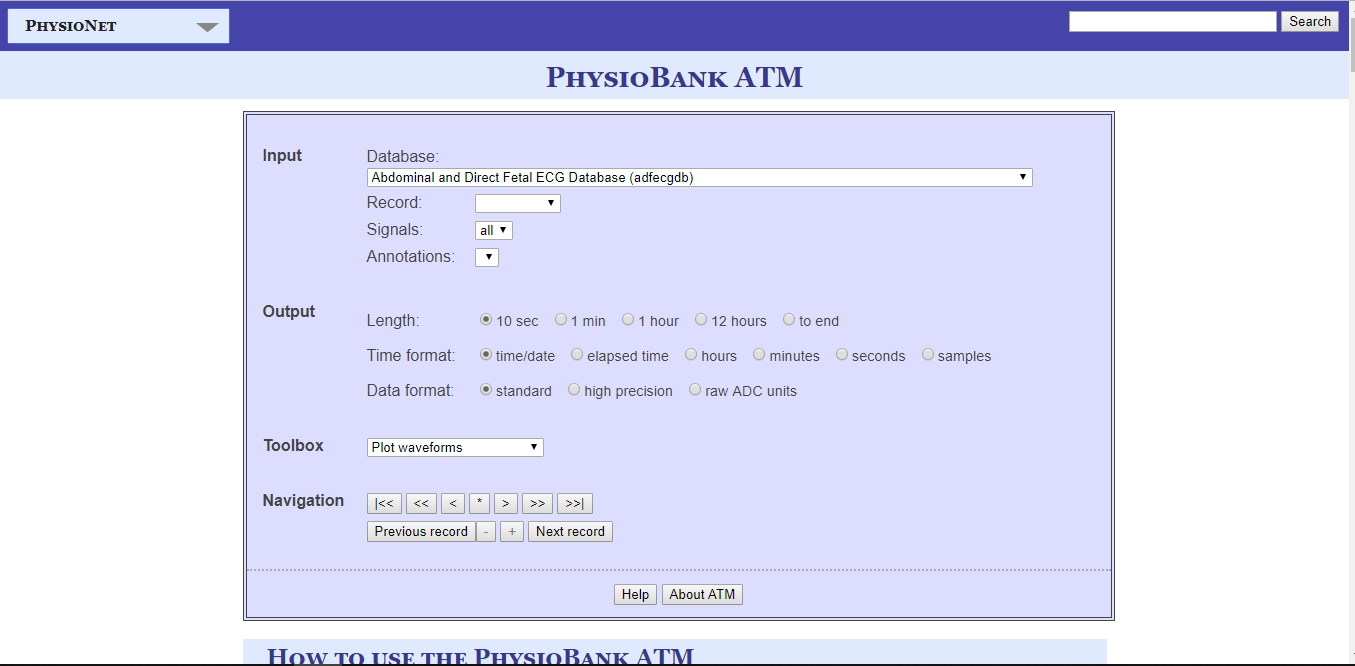
\includegraphics[scale=.3]{image/chapter5/physionet_bank.png}
\begin{figure}[htp]
\begin{center}
\end{center}
\caption{Nguồn thu thập dữ liệu online}
\end{figure}
\end{center}
Bộ dữ liệu được sử dụng: MIT-BIH arrhythmia database.\\
Những đặc điểm của dữ liệu:
\begin{itemize}
    \item Dữ liệu trong thử nghiệm được lấy trên chuyển đạo Lead II trong 2 channel của dữ liệu MIT-BIH vì chuyển đạo này thể hiện rõ ràng nhất đặc điểm của ECG.
    \item Dữ liệu sau khi qua giai đoạn lọc nhiễu và  cắt đoạn RR thu được 98872 (đoạn RR) bao gồm (51765 bình thường và 47107 bất thường)
\end{itemize}
\begin{center}
    \begin{tabular}{|c|c|}
    \hline 
    Tập dữ liệu huấn luyện & Tập dữ liệu kiểm thử \\ 
    \hline 
    79153 & 19719\\ 
    \hline 
    \end{tabular}
\end{center}

\subsection{Kết quả}
Độ chính xác của quá trình phân loại (accuracy): 0.916 và Độ mất mát của quá trình phân loại (loss): 0.052.
\subsection{Đánh giá}
\begin{itemize}
    \item Độ chính xác của mô hình phân loại chưa được cao như những nghiên cứu khác.
\end{itemize}
\subsection{Trở ngoại}
\begin{itemize}
    \item Chỉ mới áp dụng mô hình phân loại trên chuyển đạo Lead II.
    \item Những vấn đề trong việc xử lý dữ liệu, nhiễu...
\end{itemize}


\chapter{Tổng kết và hướng phát triển}
\newpage

\section{Tổng kết}
Mô hình thực hiện đã dùng các kỹ thuật học sâu: LSTM để thực hiện phân loại và phát hiện bất thường ở ECG .Bên cạnh đó có sử dụng những kỹ thuật signal processing để xử lý tín hiệu điện tâm đồ. Việc phát hiện sớm và điều trị giúp giảm thiểu nguy cơ mắc bệnh tim mạch.

\section{Hướng phát triển}
\begin{itemize}
    \item Mở rộng nguồn dữ liệu, kết hợp nhiều nguồn dữ liệu.
    \item Nghiên cứu phân loại trên những chuyển đạo khác để có những kết quả toàn diện hơn.
    \item Thử nghiệm nhiều mô hình phân loại khác, nghiên cứu và cải tiến để thu được mô hình phân loại tốt nhất
    \item Mở rộng phân loại từng nhóm bệnh cụ thể khi phát hiện có bất thường.
\end{itemize}

%-	Danh mục TL tham khảo
%-	Phụ lục (nếu có)
%tham khao
%nothing here
\bibliographystyle{plain}
\bibliography{ref.bib}
\end{document}